\documentclass[letterpaper, 10pt, dvipsnames]{article}
\usepackage[utf8]{inputenc}
\usepackage[T1]{fontenc}
\usepackage{float, graphicx, caption, wrapfig, tikz}
\usepackage{amsthm, amsmath, amsfonts, amssymb, mathrsfs, mathtools}
\usepackage{hyperref, xcolor, titlesec}

\begin{document}

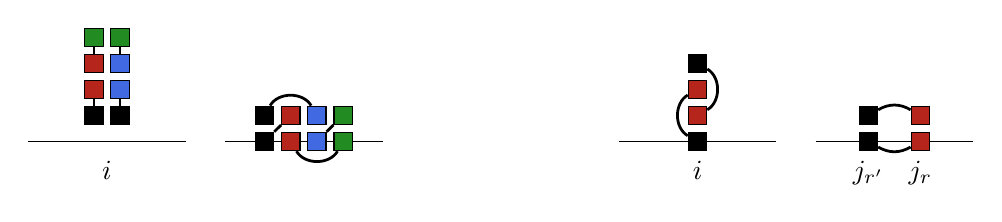
\begin{tikzpicture}
		\draw[black] (-1,0) -- (1,0);
		\node[draw=none,black,label=below:\textcolor{black}{$i$}] at (0,0) {};
		
		\node[draw,black,fill=black] (1) at (-0.165,0.33) {};
		\node[draw,black,fill=BrickRed] (2) at (-0.165,0.66) {};
		\node[draw,black, fill=BrickRed] (3) at (-0.165,0.99) {};
		\node[draw,black, fill=ForestGreen] (4) at (-0.165,1.32) {};
		
		\node[draw,black,fill=black] (11) at (0.165,0.33) {};
		\node[draw,black,fill=RoyalBlue] (12) at (0.165,0.66) {};
		\node[draw,black, fill=RoyalBlue] (13) at (0.165,0.99) {};
		\node[draw,black, fill=ForestGreen] (14) at (0.165,1.32) {};
		
		\path[-, black,line width=.1em] (11) edge (12);
		\path[-, black,line width=.1em] (1) edge (2);
		\path[-, black,line width=.1em] (13) edge (14);
		\path[-, black,line width=.1em] (3) edge (4);
		
		
		\begin{scope}[xshift=2.5cm]
			\draw[black] (-1,0) -- (1,0);
			\node[draw,black,fill=black] (1) at (-0.5,0.33) {};
			\node[draw,black,fill=black] (2) at (-0.5,0) {};
			\node[draw,black, fill=BrickRed] (3) at (-0.165,0) {};
			\node[draw,black, fill=BrickRed] (4) at (-0.165,.33) {};
			
			\node[draw,black,fill=RoyalBlue] (11) at (0.165,0.33) {};
			\node[draw,black,fill=RoyalBlue] (12) at (0.165,0) {};
			\node[draw,black, fill=ForestGreen] (13) at (0.5,0) {};
			\node[draw,black, fill=ForestGreen] (14) at (0.5,.33) {};
			
			\path[-, black,line width=.1em] (2) edge (4);
			\path[-, black,line width=.1em] (3) edge[bend right=60] (13);
			\path[-, black,line width=.1em] (12) edge (14);
			\path[-, black,line width=.1em] (11) edge[bend right=60] (1);
		\end{scope}
		\begin{scope}[xshift=7.5cm]
			\draw[black] (-1,0) -- (1,0);
			
			\node[draw,black, fill=black, label=below:$\textcolor{black}{i}$] (1) at (0,0) {};
			\node[draw,black, fill=BrickRed] (2) at (0,.33) {};
			\node[draw,black, fill=BrickRed] (3) at (0,.66) {};
			\node[draw,black, fill=black] (4) at (0,.99) {};
			
			\path[-,black,line width=.1em] (1) edge[bend left=60] (3);
			\path[-,black,line width=.1em] (4) edge[bend left=60] (2);
			
			\begin{scope}[xshift = 2.5cm]
				\draw[black] (-1,0) -- (1,0);
				
				\node[draw,black,fill=black, label=below:$\textcolor{black}{j_{r'}}$] (11) at (-0.33,0) {};
				\node[draw,black,fill=black,] (12) at (-0.33,.33) {};
				\node[draw,black, fill=BrickRed, label=below:$\textcolor{black}{j_{r}}$] (13) at (0.33,.0) {};
				\node[draw,black, fill=BrickRed] (14) at (0.33,.33) {};
				
				\path[-, black,line width=.1em] (11) edge[bend right=30] (13);
				\path[-, black,line width=.1em] (12) edge[bend left=30] (14);
			\end{scope}
			
		\end{scope}
	\end{tikzpicture}

\end{document}